\documentclass{article}
\usepackage[a4paper]{geometry}
\usepackage[utf8]{inputenc}
\DeclareUnicodeCharacter{00A0}{ }
\usepackage[english, italian]{babel}
\usepackage{parskip}
\usepackage{etaremune}
\usepackage{appendix}
\renewcommand\appendixtocname{Appendici}
\setcounter{secnumdepth}{4}
\setcounter{tocdepth}{4}
\usepackage[usenames,dvipsnames]{color}
\usepackage{titlesec}
\usepackage{float}
\usepackage[colorlinks=true]{hyperref}
\hypersetup{
    colorlinks=true,
    citecolor=black,
    filecolor=black,
    linkcolor=black,
    urlcolor=blue
}
\usepackage{breakurl}
\usepackage{graphicx}
\usepackage{lastpage}
\usepackage{longtable}
\usepackage{booktabs}
\usepackage{tabularx}
\usepackage{multirow}
\usepackage{longtable}
\usepackage[table]{xcolor}
\usepackage{tabu}
\setlength{\tabulinesep}{6pt}
\usepackage{array}
\usepackage{ragged2e}
\newcolumntype{P}[1]{>{\RaggedRight\hspace{0pt}}p{#1}}
\usepackage{fancyhdr}
\usepackage{textcomp}
\usepackage{changepage}
\usepackage{pgfplots}
\usepackage{tikz}
\usepackage{grffile}
\usepackage{rotating}
\usepackage{calc}
\fancypagestyle{plain}{
	% cancella tutti i campi di intestazione e piè di pagina
	\fancyhf{}

	\lhead{
		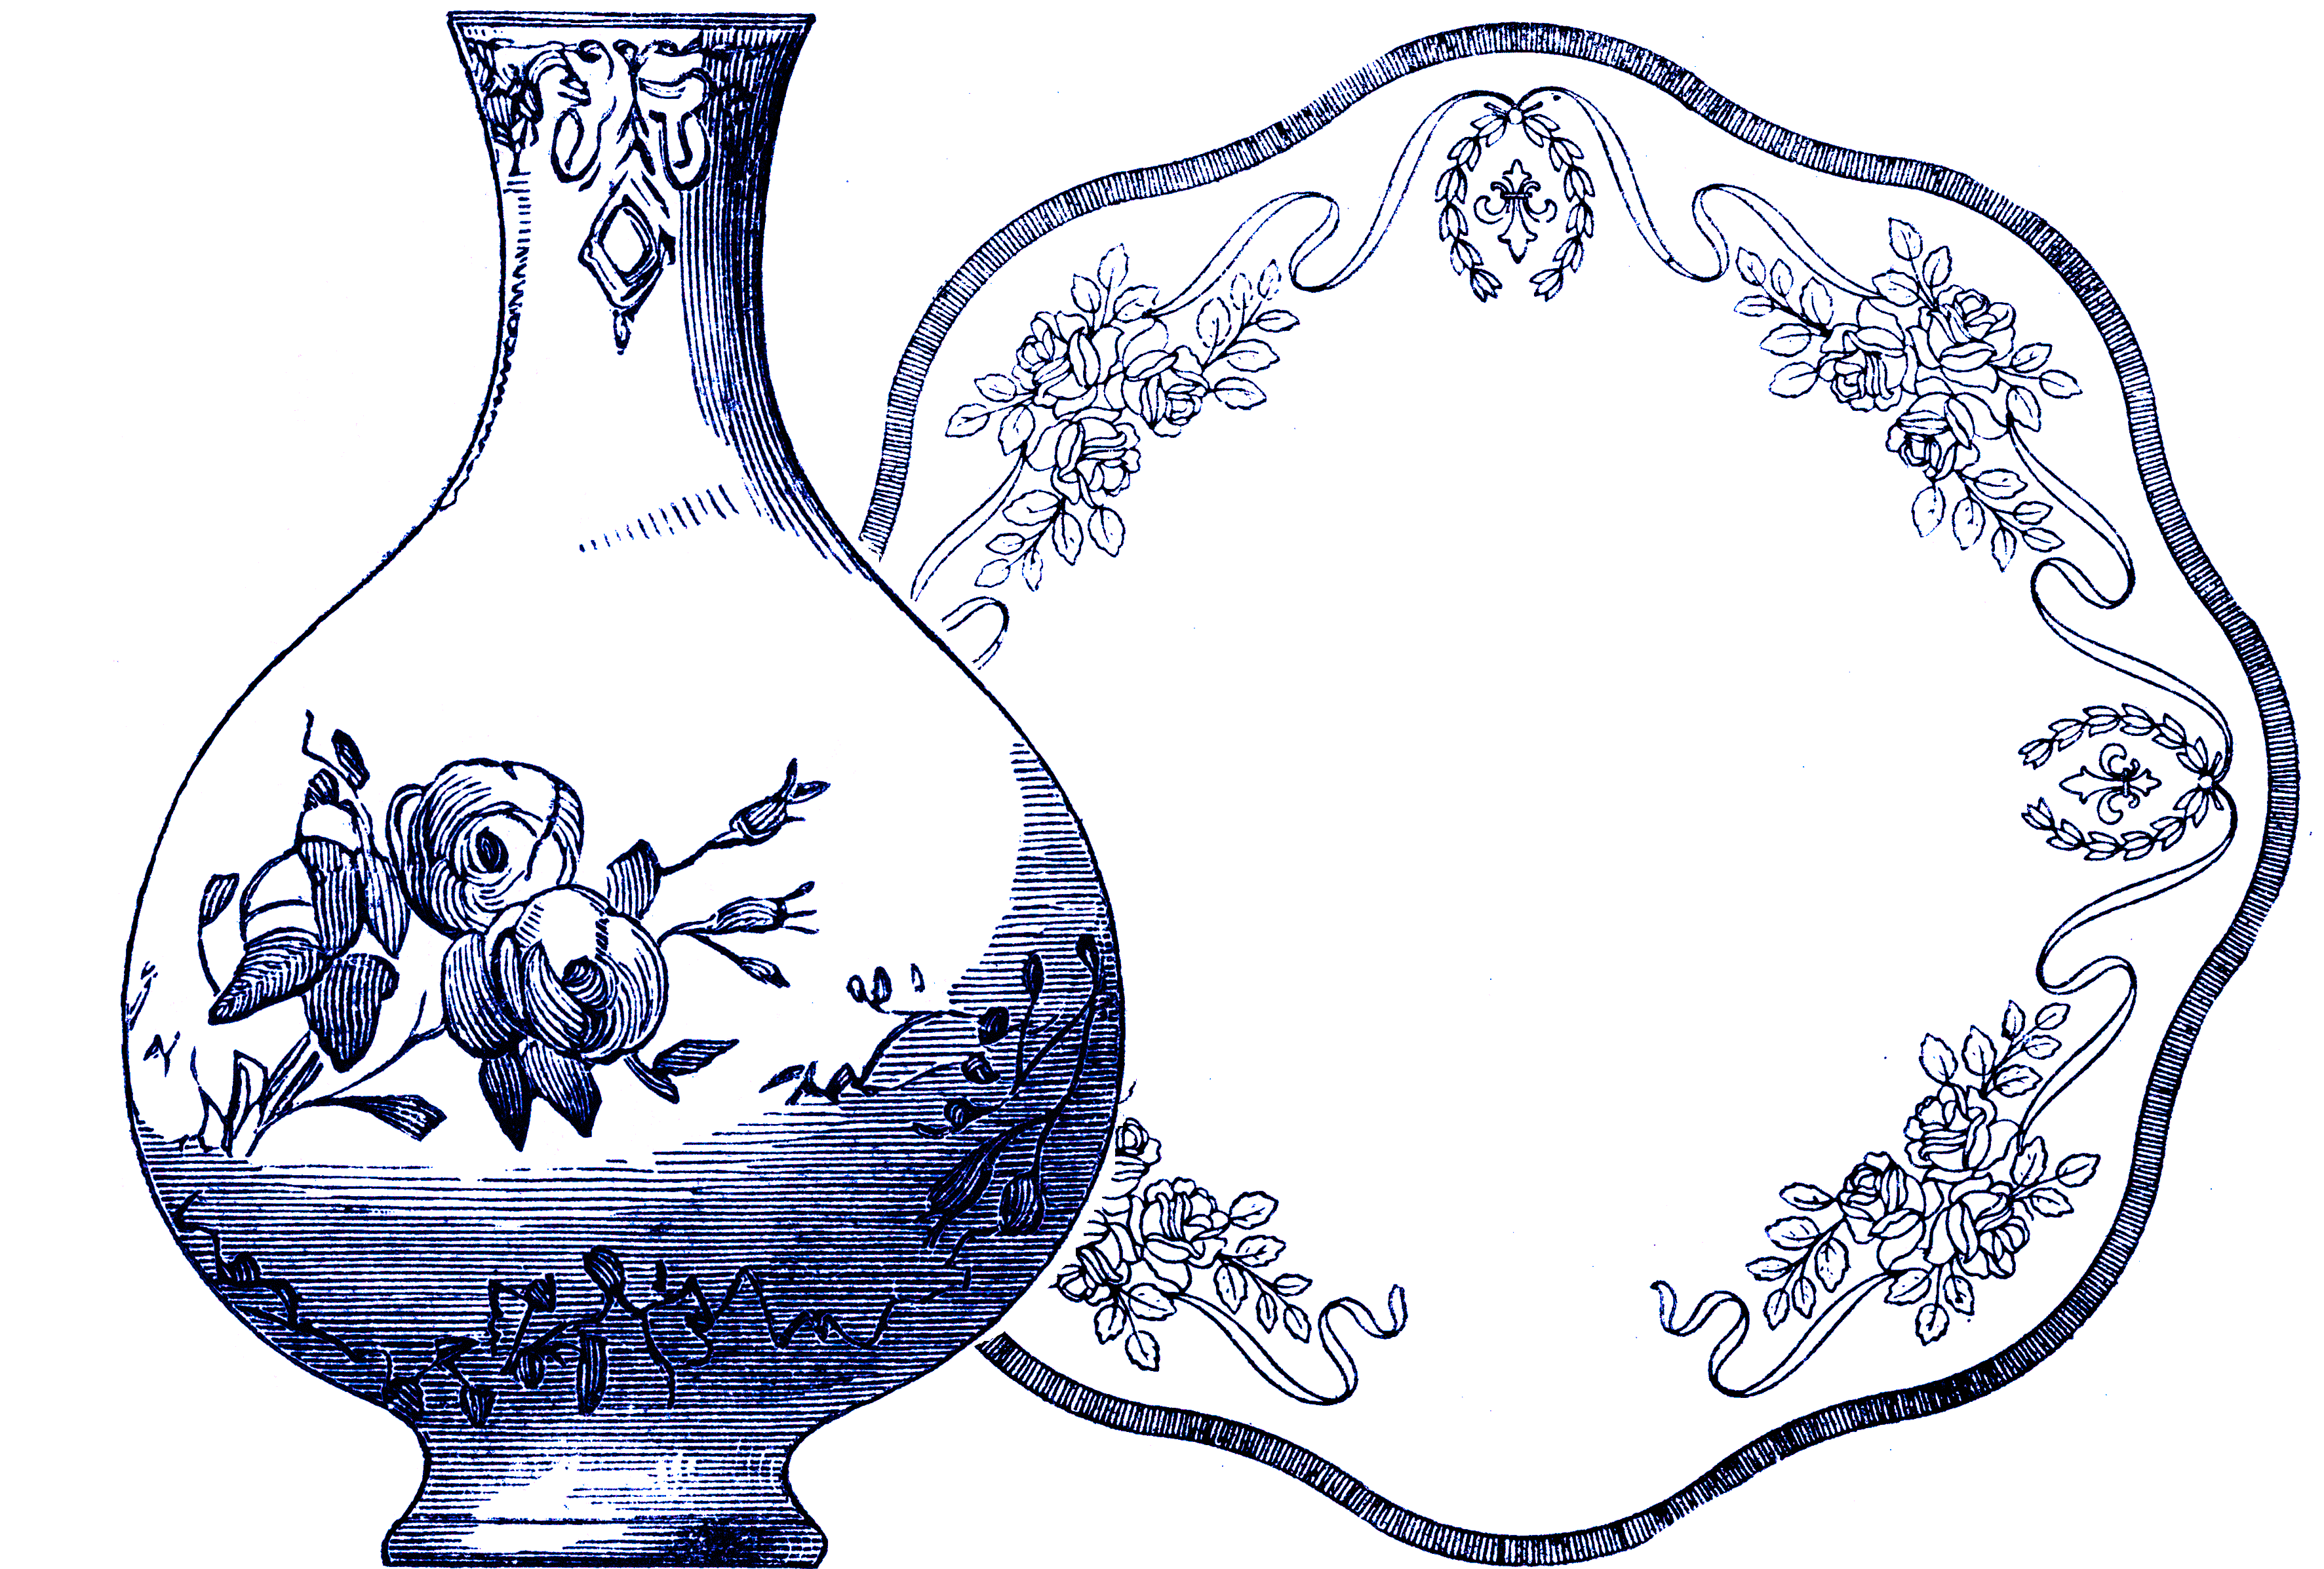
\includegraphics[height=1.5cm, width=1.5cm, keepaspectratio=true]{logo.png}
		\parbox[b]{10cm}{
			\emph{\ProjectName{}} \vspace{7pt}
		}
	}
	\chead{}
	\rhead{
		\slshape \leftmark
	}

	\lfoot{
		\ProjectName{}
	}
	\rfoot{Pagina \thepage{} di \pageref{LastPage}}
	\renewcommand{\headrulewidth}{0.3pt}
	\renewcommand{\footrulewidth}{0.3pt}
}
\setlength{\headheight}{30pt}
\pagestyle{plain}
\usepackage{listings}
\lstset{
  extendedchars=true,          % lets you use non-ASCII characters
  inputencoding=utf8,   % converte i caratteri utf8 in latin1, richiede \usepackage{listingsutf8} anzichè listings
  basicstyle=\ttfamily,        % the size of the fonts that are used for the code
  breakatwhitespace=false,     % sets if automatic breaks should only happen at whitespace
  breaklines=true,             % sets automatic line breaking
  captionpos=t,                % sets the caption-position to top
  commentstyle=\color{mygreen},   % comment style
  frame=none,               % adds a frame around the code
  keepspaces=true,            % keeps spaces in text, useful for keeping indentation of code (possibly needs columns=flexible)
  keywordstyle=\bfseries,     % keyword style
  numbers=none,               % where to put the line-numbers; possible values are (none, left, right)
  numbersep=5pt,              % how far the line-numbers are from the code
  numberstyle=\color{mygray}, % the style that is used for the line-numbers
  rulecolor=\color{black},    % if not set, the frame-color may be changed on line-breaks within not-black text (e.g. comments (green here))
  showspaces=false,           % show spaces everywhere adding particular underscores; it overrides 'showstringspaces'
  showstringspaces=false,     % underline spaces within strings only
  showtabs=false,             % show tabs within strings adding particular underscores
  stepnumber=5,               % the step between two line-numbers. If it's 1, each line will be numbered
  stringstyle=\color{red},    % string literal style
  tabsize=4,                  % sets default tabsize
  firstnumber=1      % visualizza i numeri dalla prima linea
}
\usepackage[T1]{fontenc}
\usepackage{lmodern}
\newcommand{\ProjectName}{LineaCasaBari}

\newcommand{\makeFrontPage}{
  % Declare new goemetry for the title page only.
  \newgeometry{top=3.5cm}
  
  \begin{titlepage}
  \begin{center}

  \begin{center}
  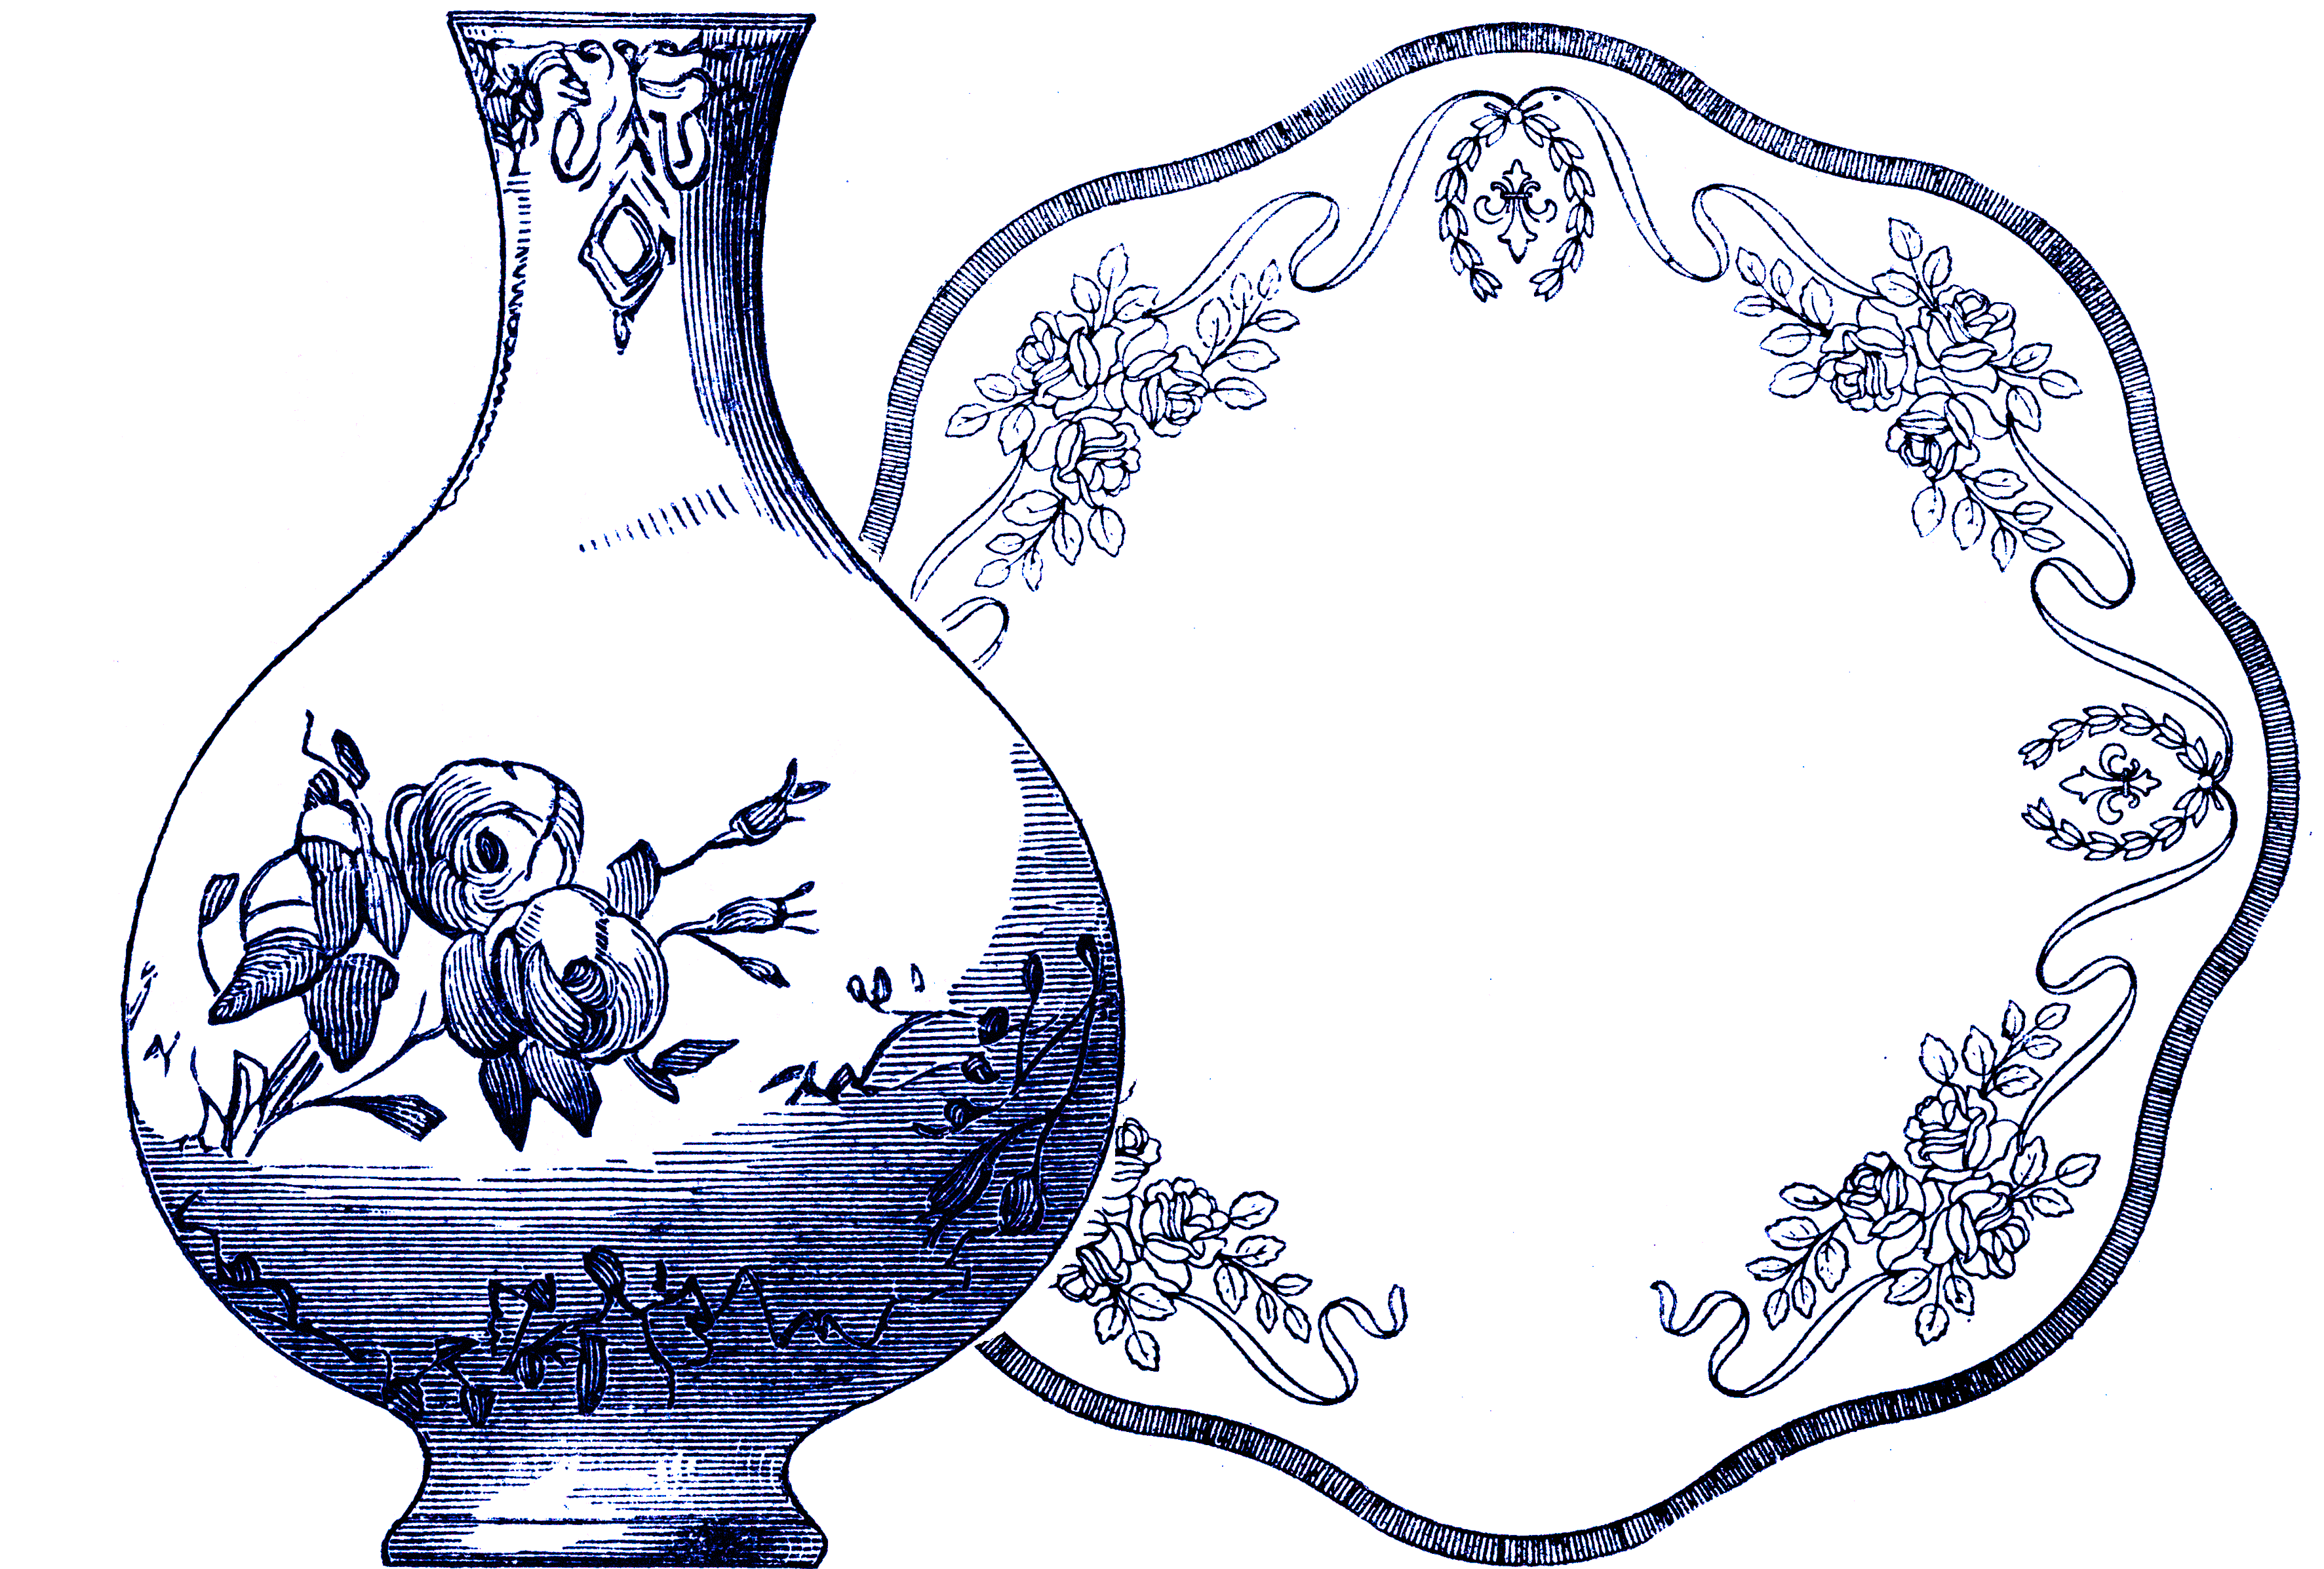
\includegraphics[width=10cm]{logo.png}
  \end{center}
  
  \vspace{1cm}

  \begin{Huge}
  \textbf{\ProjectName{}}
  \end{Huge}
  
  \vspace{11pt}

  \bgroup
  \def\arraystretch{1.3}
  \begin{tabular}{ r|l }
    \multicolumn{2}{c}{\textbf{Membri del gruppo}} \\
    \hline

    \textbf{Navid Taha} & 1069126 \\
    \textbf{Alice Sasso} & 1074588 \\
    \textbf{Lorenzo Ferrarin} & 1069405 \\
    \textbf{Alessandro Bari} & 1074356 \\
  \end{tabular}
  \egroup

  \vspace{22pt}

  \textbf{Informazioni sul sito} \\
  
  	\url{http://tecnologie-web.studenti.math.unipd.it/tecweb/~asasso/}
  	
  \vspace{5pt}
  \textbf{Referente} \\
  Navid Taha: navid.taha@studenti.unipd.it
  
  \vspace{7pt}  
  
  \textbf{Dati di accesso} \\
  
  
  
  login amministratore e utente
    
  
  \end{center}
  \end{titlepage}
  
  % Ends the declared geometry for the titlepage
  \restoregeometry
}

\begin{document}

\makeFrontPage
\clearpage
\tableofcontents
\listoffigures
\clearpage

\section{Riferimenti informativi}

\section{Introduzione}
Il progetto ha lo scopo di sviluppare il sito web commerciale del negozio LineaCasaBari, operante nel settore della vendita di oggetti per la casa. \\
Il sito sarà composto da due principali aree: utente ed amministratore. \\
L'area amministratore consentirà la gestione del sito, tramite diverse funzionalità quali la rimozione di un utente, la rimozione/aggiunta/modifica di un prodotto, la modifica di un ordine e la rimozione/aggiunta/modifica di un annuncio. \\
L'area utente consentirà la consultazione un elenco di prodotti acquistabili, la gestione del proprio account (modifica dei dati e degli indirizzi associati) e la visualizzazione di informazioni nel sito, tramite annunci e sezioni predisposte. \\
Lo sviluppo del sito è stato conferme alle predisposizioni degli standard W3C, ed inoltre si è mantenuta la separazione tra comportamento, struttura e presentazione.

\section{Analisi dei requisiti} % individuazione degli utenti e delle loro esigenze
	\subsection{Utenti esterni}
		\subsubsection{Utente non registrato}
		L'utente non registrato deve poter consultare il catalogo dei prodotti, tuttavia per l'acquisto dei prodotti dovrà registrarsi. Inoltre, ha la possibilità di consultare diverse informazioni, sia sui servizi proposti, che in generale sul sito e sulle novità di esso.  \\
		Le informazioni che cerca devono essere accessibili nel minor numero di click, in quanto è stato riscontrato che la permanenza di utente nel sito dipende da quanto tempo è necessario per reperire le informazioni utili.
		
		\subsubsection{Utente registrato}
		L'utente registrato visualizza la stessa versione del sito dell'utente non registrato, in modo da favorirne l'orientamento in esso. Tuttavia, ha la possibilità di effettuare degli ordini ed acquistare i prodotto offerti dal negozio. Inoltre, ha accesso alla sezione di gestione del proprio account, in cui ha la possibilità di modificare i dati del proprio account, aggiungere/modificare/rimuovere gli indirizzi di spedizione e %annullare
		consultare gli ordini effettuati; è presente anche la lista dei desideri, in cui l'utente può salvare i suoi articoli preferiti in modo da ritrovarli successivamente.

	\subsection{Utenti interni}
		\subsubsection{Amministratore}
		L'amministratore è la figura che gestisce il sito e lo mantiene. Si presume che non abbia intenzioni malevole verso di esso e che sia una persona esperta in tale ambito. Nonostante, sono stati previsti dei controlli, in modo da evitare eventuali distrazioni ed errori. \\
		L'amministratore ha la possibilità di gestire il sito effettuando l'accesso con delle credenziali speciali, immesse direttamente nel database dell'applicativo, nello stesso form di login utilizzato dagli utenti. Potrà successivamente accedere alla sezione di gestione del sito tramite un link posto nell'intestazione del sito. In tale sezione, è possibile gestire (modifica/ rimozione/ aggiunta) i dati del database interno del sito, che sono rappresentati dagli utenti, ordini, prodotti e annunci. \\
		Vengono mantenute le funzionalità offerte agli utenti, in modo da poterne verificare il funzionamento e la correttezza dal punto di vista dell'utente stesso, senza il bisogno di creare un altro account.

\section{Dati e informazioni} % progettazione della base informativa
	\subsection{Contenuti}
	Il sito ha la necessità di salvare e reperire, da un'apposita base di dati XML, i seguenti dati:
	\begin{itemize}
		\item \textbf{Annunci}: rappresentano i messaggi contenenti novità ed informazioni riguardanti il negozio. La gestione di questi dati viene riservata all'amministratore;
		\item \textbf{Utenti}: rappresentano gli utenti iscritti al sistema, compresi gli amministratori. Gli amministratore vengono individuati da un campo booleano e devono essere aggiunti a mano, modificando il file XML. La gestione di questi dati viene riservata all'amministratore;
		\item \textbf{Prodotti}: rappresentano i prodotti offerti dal negozio ed acquistabili dagli utenti registrati. La gestione di questi dati viene riservata all'amministratore;
		\item \textbf{Indirizzi}:
	\end{itemize}
\section{Applicazioni e servizi} % progettazione delle funzionalità

\section{Accessibilità e stile} % progettazione dell'organizzazione

\section{Strumenti e manutenzione} % Progettazione fisica

\end{document}